\subsection{Distance Estimation}

After the intrinsic matrix for the recording has been calculated, the approximate distance to the object can now be calculated with the assumptions made in chapter \ref{obj}. However, this is only an estimated distance, since the coefficients of the intrinsic matrix are subjected to noise depending on the recordings and the used images for the calibration.\\

To do this, an image is first created that clearly shows the object in the desired distance with the object. In this case the last frame of the \textit{'250\_cm\_distance.h264’}-recording was taken and an undistorted image was generated from it with the calculated intrinsic matrix and distortion coefficients. The result can be seen in figure \ref{fig:250_og}.\\

From this image, two boundary points are now determined that lie on the edge of the checkerboard and on a straight line. The boundary points are marked as green points in figure \ref{fig:250_green}. In the same process the pixel coordinates $(z_1, z_2)^{T}$ can be noted for both boundary points.\\

\begin{figure}[H]
     \centering
     \captionsetup{justification=centering}
     \begin{minipage}[t]{0.5\textwidth}
        \centering
        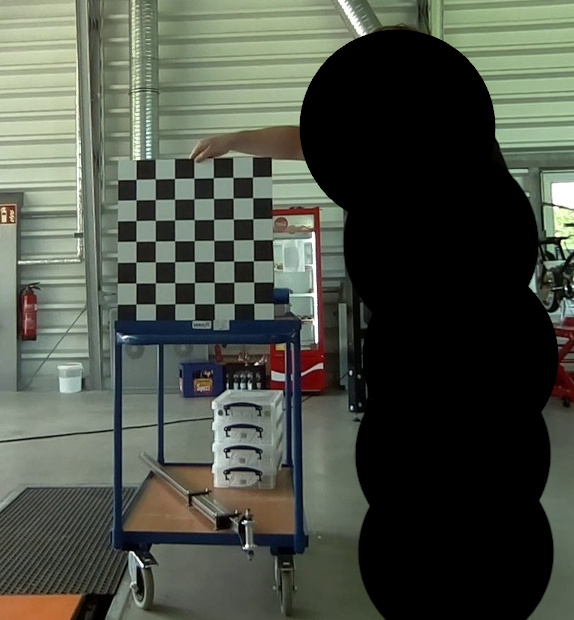
\includegraphics[width=.95\textwidth]{image/2/250_undist_cropped.jpg}
        \caption{Undistorted and cropped image}
        \label{fig:250_og}
     \end{minipage}%
     \begin{minipage}[t]{0.5\textwidth}
        \centering
        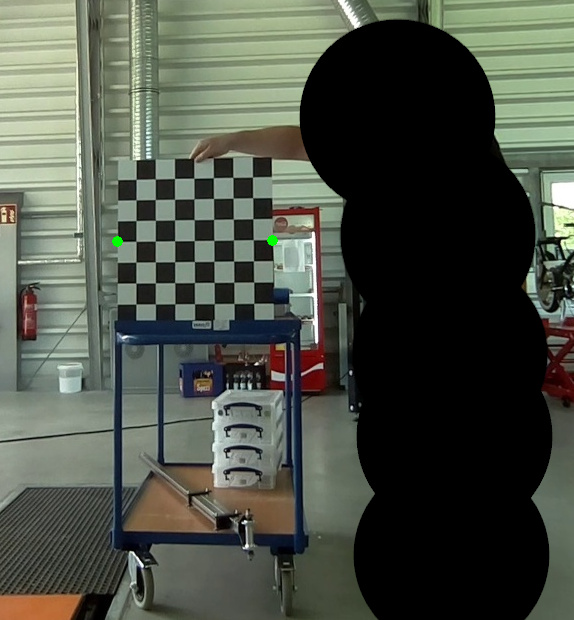
\includegraphics[width=.95\textwidth]{image/2/250_undist_cropped_green.jpg}
        \caption{Boundary points \textit{A} and \textit{B} \\in green colour}
        \label{fig:250_green}
     \end{minipage}
\end{figure}

\newpage 
With the pixel coordinates $(z_1, z_2)^{T}$ and the intrinsic matrix $\bm{K}$ one can calculate the \\ simplified full line $\vec{L}$ between camera and pixel coordinate. The equation can be seen in equation \ref{eq:1}. The calculated line $z \vec{\lambda}$ is filled with potential distance positions $z$.

{\large
\begin{equation}\label{eq:1}
    \vec{L} = \left \{ 
            \begin{pmatrix}
                \lambda_1\\ 
                \lambda_2\\ 
                \lambda_3
            \end{pmatrix} 
            \in \mathbb{R}^{3}\text{;}\;
            z \! \begin{pmatrix}
                \lambda_1\\ 
                \lambda_2\\ 
                \lambda_3
            \end{pmatrix} 
            = z\bm{k}
            \begin{pmatrix}
                z_1\\ 
                z_2\\ 
                1
            \end{pmatrix} 
            \text{and} \; z \in \mathbb{R}\right \}
            \text{with} \; \bm{k} = \bm{K^{-1}}
\end{equation}
}
\vspace{2mm}

%\newpage

With the equation \ref{eq:1} and the known boundary points \textbf{A} and \textbf{B} with pixel coordinates $(z_1, z_2)^{T}$ one can calculate the corresponding vectors $\vec{a}$ and $\vec{b}$ shown in equation \ref{eq:2_1} and \ref{eq:2_2}.

{\large
\begin{align}\label{eq:2_1}
    \vec{a}(z) &= z \vec{\lambda_A} = z \! 
    \begin{pmatrix}
        \lambda_{1A}\\ 
        \lambda_{2A}\\ 
        \lambda_{3A}
    \end{pmatrix} = z\bm{k}
    \begin{pmatrix}
        A_x\\ 
        A_y\\
        1
    \end{pmatrix} = z\bm{k}
    \begin{pmatrix}
        z_{1A}\\ 
        z_{2A}\\
        1
    \end{pmatrix}\\[10pt]
    \vec{b}(z) &= z \vec{\lambda_B} = z \! 
    \begin{pmatrix}
        \lambda_{1B}\\ 
        \lambda_{2B}\\
        \lambda_{3B}
    \end{pmatrix} = z\bm{k}
    \begin{pmatrix}
        B_x\\ 
        B_y\\
        1
    \end{pmatrix}= z\bm{k}
    \begin{pmatrix}
        z_{1B}\\ 
        z_{2B}\\
        1
    \end{pmatrix}\label{eq:2_2}
\end{align}
}

\begin{wrapfigure}[19]{L}{0.57\textwidth}
    \vspace{\baselineskip}
    \centering
     \captionsetup{justification=centering}
     \begin{minipage}[b]{0.55\textwidth}
         \centering
         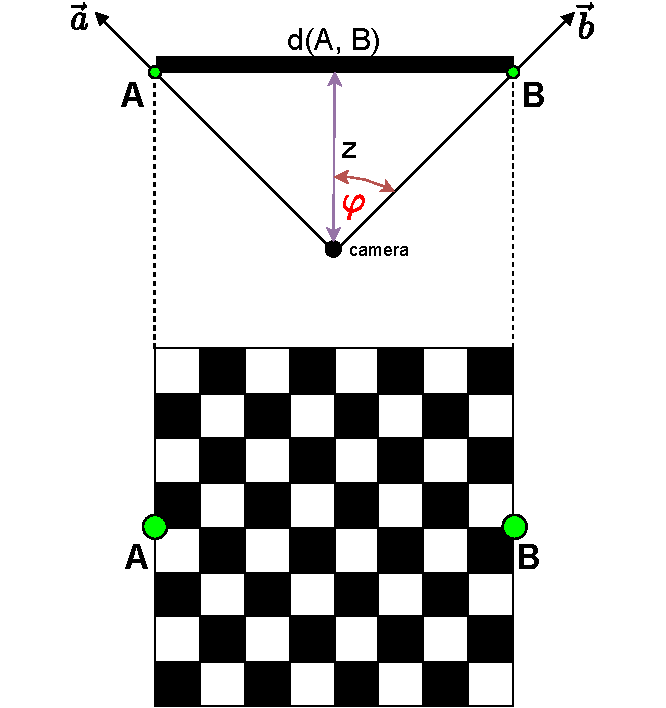
\includegraphics[width=\textwidth]{image/2/calc_line.pdf}
         \caption{Visualisation of the relationships}
         \label{fig:calc_line}\par
     \end{minipage}

\end{wrapfigure}

\newpage
These relationships are shown again in figure \ref{fig:calc_line}. \\The vectors $\vec{a}$ and $\vec{b}$ and the known size of the checkerboard $d(A, B)$ are defining a triangular area based on the assumptions  made in chapter \ref{obj}. \\

Since one assumption is that the checkerboard is perpendicular to the camera, we can assume that the vectors $\vec{a}$ and $\vec{b}$ have the same angle to the camera. Thus we can calculate the distance $z$ of the resulting triangle if the norms $|\vec{a}(z)|=|\vec{b}(z)|$ with a distance between the vectors of $d(A, B)$. For this one can use the trigonometric formulas if the angle between both vectors is known.\\

The angle $\varphi_{tot}$ between two vectors can be calculated using the dot product.
\vspace{-2mm}
{\large % change font size
% https://de.overleaf.com/learn/latex/Spacing_in_math_mode
\begin{align}
    \varphi_{tot} &= \arccos{\frac{\vec{a} \cdot \vec{b}}{|\vec{a}||\vec{b}|}}\nonumber\\[5pt]
    \varphi_{tot} &= 2\varphi = \arccos{\frac{\vec{\lambda_A} \cdot \vec{\lambda_B}}{|\vec{\lambda_A}||\vec{\lambda_B}|}}\nonumber\\[5pt]
    \Rightarrow \varphi &= \frac{1}{2}\arccos{\frac{\vec{\lambda_A} \cdot \vec{\lambda_B}}{|\vec{\lambda_A}||\vec{\lambda_B}|}}\label{eq3}
    % d(A, B)^{2} &= (z \lambda_{1A} - z \lambda_{1B})^{2} + (z \lambda_{2A} - z \lambda_{2B})^{2}\\
    % d(A, B)^{2} &= z^{2}(kA_x - kB_x)^{2} + z^{2}(kA_y - kB_y)^{2}\\
    % d(A, B)^{2} &= z^{2}[(\overset{\thicksim}{A_x} - \overset{\thicksim}{B_x})^{2} + \overset{\thicksim}{A_y} - \overset{\thicksim}{B_y})^{2}]
\end{align}
}

\newpage

With the calculated angle $\varphi$ one can calculate the distance $z$ using the trigonometric formulas. 
{\large
\begin{align}
    \tan{\varphi} &= \frac{\frac{d(A, B)}{2}}{z}\nonumber\\
    \Rightarrow z &= \frac{d(A, B)}{2\tan{\varphi}}\label{eq4}
    % (50cm)^{2} &= z^{2}\cdot x \nonumber\\
    % z &= \sqrt{\frac{(50)^2}{x}}\;cm \label{eq3}
\end{align}
}

With the intrinsic matrix $\bm{K}$, the boundary points \textbf{A} and \textbf{B}, the known size of the checkerboard $d(A, B)$ and the equations \ref{eq:2_1}, \ref{eq:2_2}, \ref{eq3} and \ref{eq4} one can calculate the estimated distance $z$ between camera and object.




